\section{Diagrammi di attività - Editor}
    \subsection{Traduzione dell'istanza dell'editor a file}
    \begin{figure}[H]
      \centering
      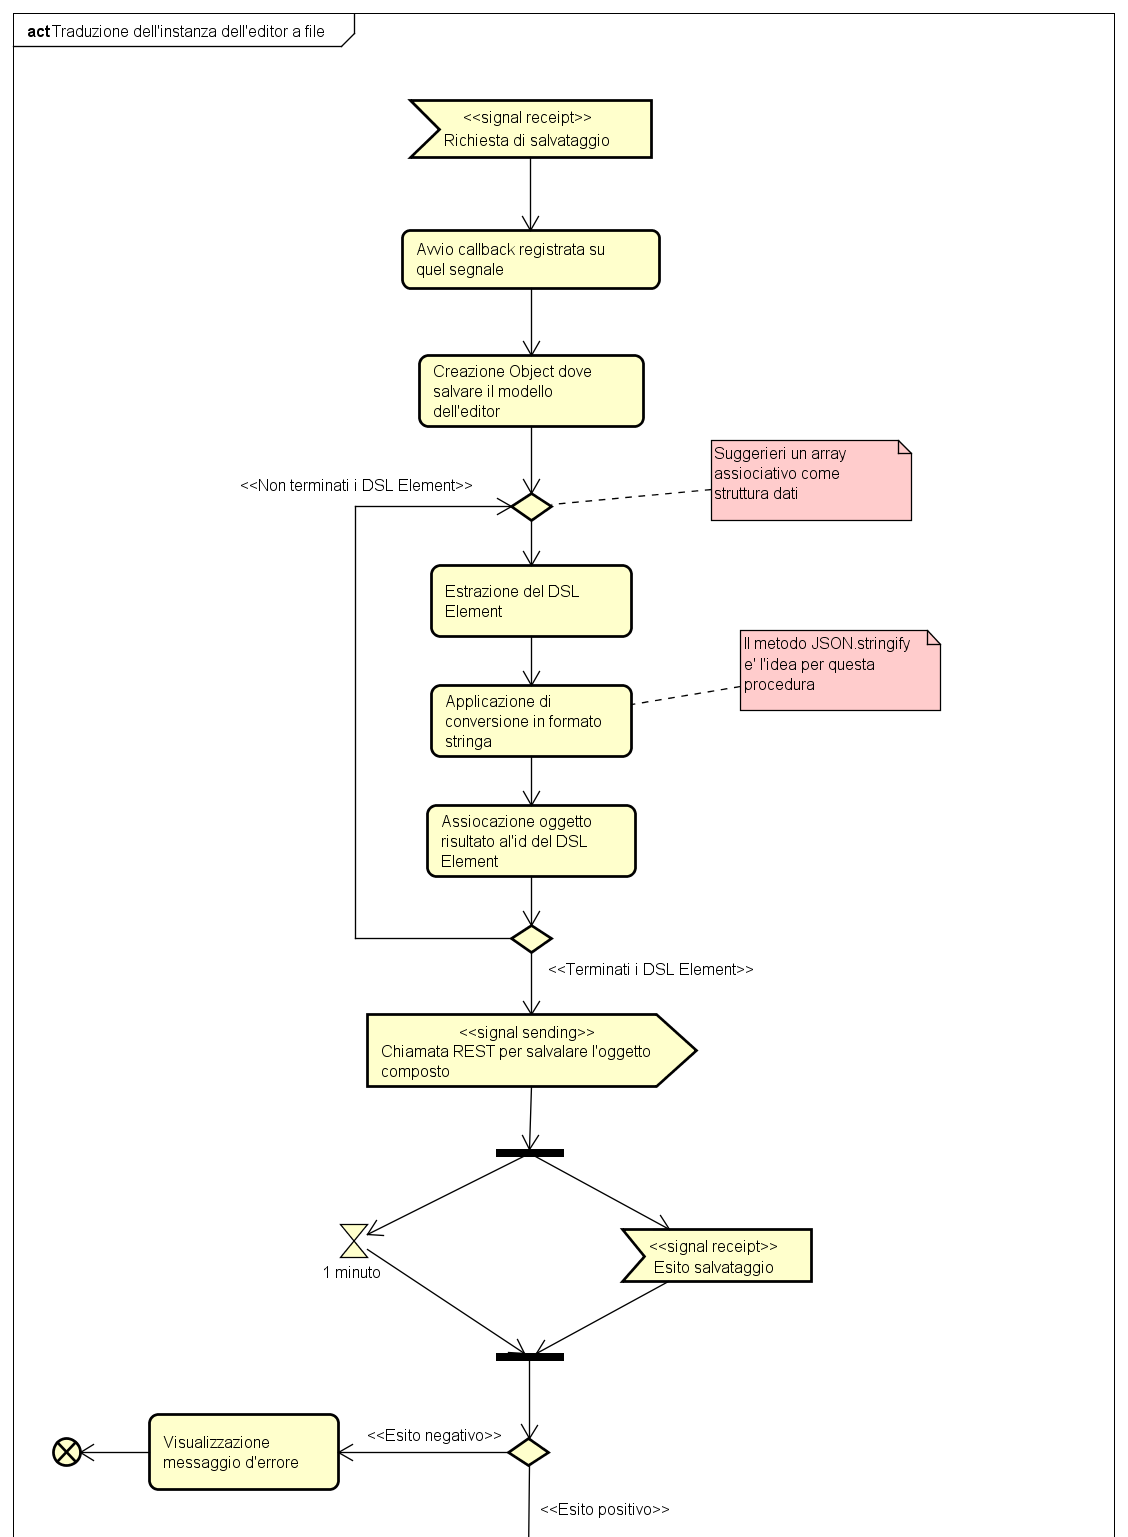
\includegraphics[width=.7\textwidth]{res/img/salvataggio.png}
      \caption{Salvataggio \glossaryItem{DSL} Structure}
      \label{fig:salvataggio}
    \end{figure}
    \begin{figure}[H]
      \centering
      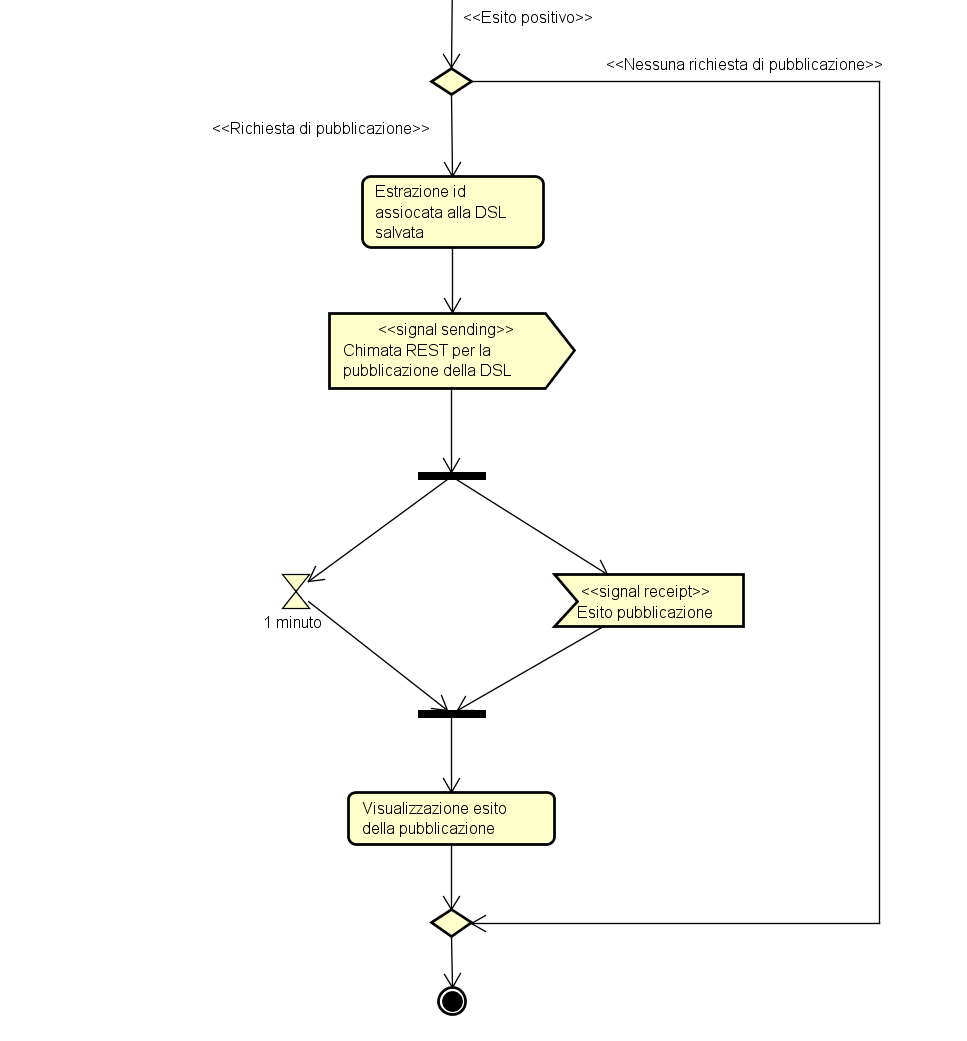
\includegraphics[width=.9\textwidth]{res/img/pubblicazione.png}
      \caption{Pubblicazione}
      \label{fig:pubblicazione}
    \end{figure}
    %L'utente puo salvare e pubblicare o salvare e non pubblicare all'inizio dell'attivita
    L'utente si trova nella pagina dell'editor e desidera salvare la specifica \glossaryItem{DSL} creata, quindi effettua una richiesta di salvataggio. Vengono convertiti in formato stringa tutti i \glossaryItem{DSL} Element presenti nel modello (la \glossaryItem{DSL} Structure) e salvati in un oggetto. Al termine, viene effettuata una chiamata \glossaryItem{REST} per salvare l'oggetto così composto e, solo in caso di esito positivo l'utente può scegliere se procedere alla pubblicazione, altrimenti termina la richiesta e viene visualizzato un messaggio di errore.
    Se l'utente desidera proseguire e pubblicare il modello \glossaryItem{DSL}, allora viene recuperato l'oggetto che lo rappresenta e viene effuttata una chiamata \glossaryItem{REST} per la pubblicazione. Al termine, viene visualizzato l'esito che sarà positivo se il modello è valido, negativo altrimenti.
    \subsection{Aggiunta di un DSL Element}
    \begin{figure}[H]
      \centering
      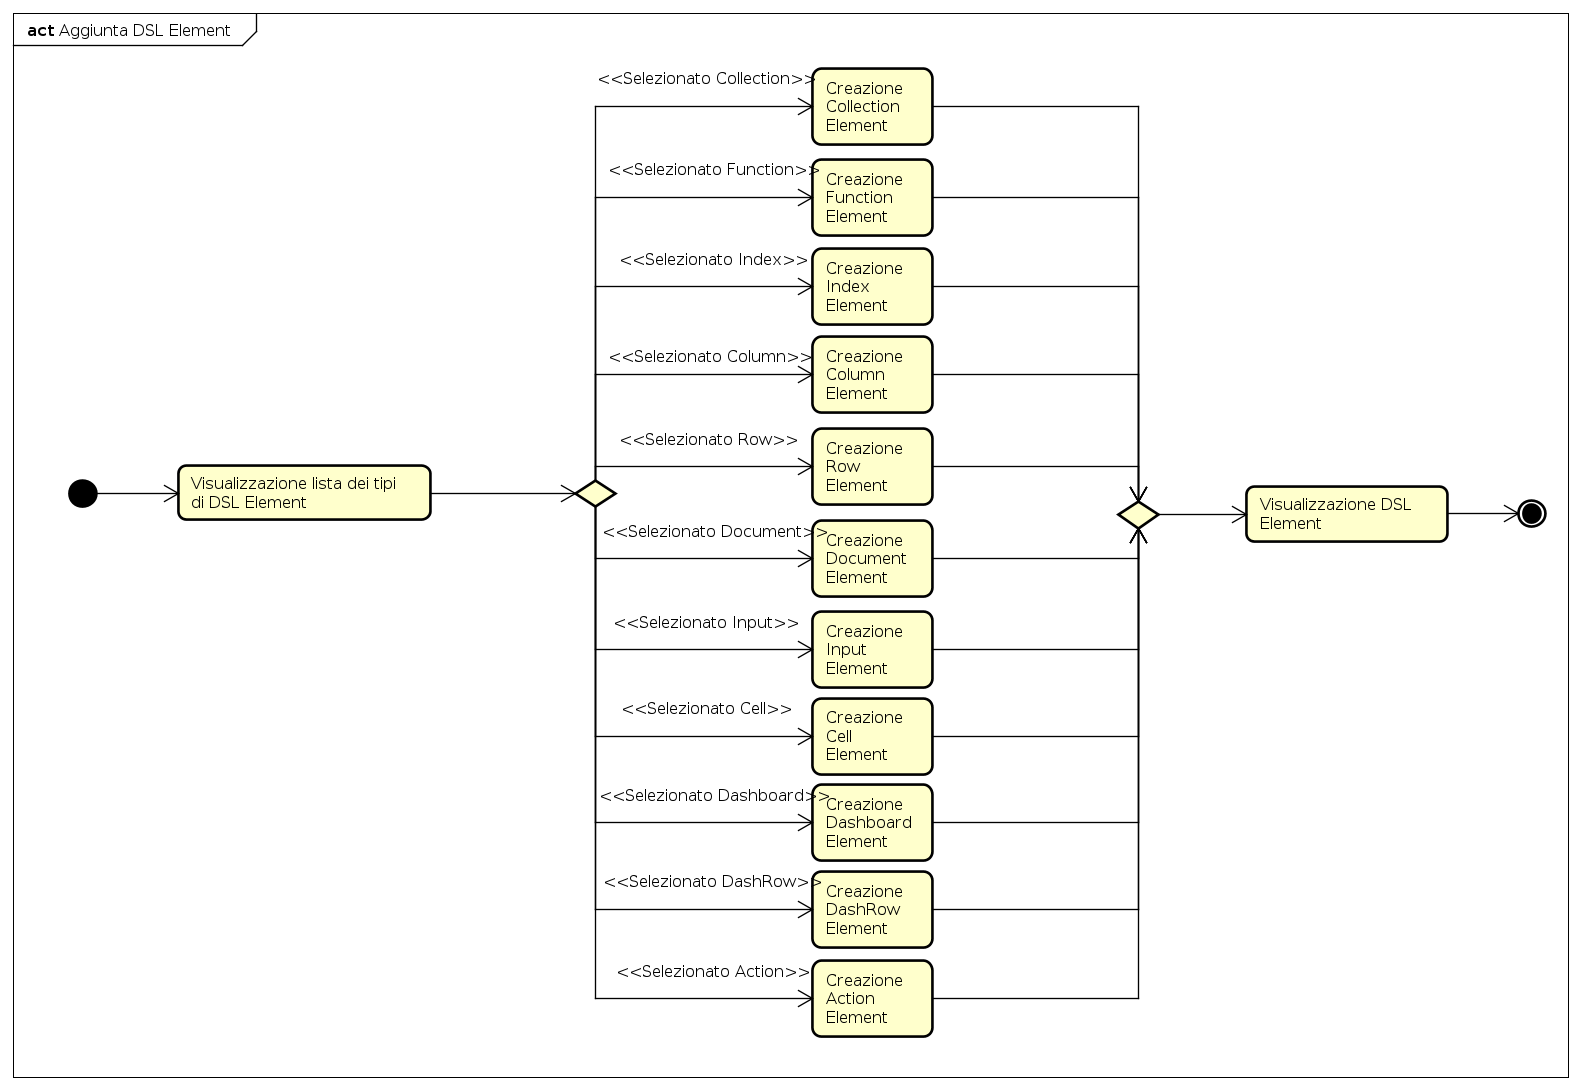
\includegraphics[width=1.0\textwidth]{res/img/aggiuntaDSLElement.png}
      \caption{Aggiunta di un \glossaryItem{DSL} Element}
      \label{fig:diagram_model}
    \end{figure}
    L'utente si trova nella pagina dell'editor e desidera creare un \glossaryItem{DSL} Element. Per prima cosa visualizza la lista dei tipi di \glossaryItem{DSL} Element disponibili, quindi seleziona quello desiderato. Viene creato il \glossaryItem{DSL} Element e l'utente può vederlo nello spazio dell'editor.
    \subsection{Associare un DSL Element ad un campo di un DSL Element}
    \begin{figure}[H]
      \centering
      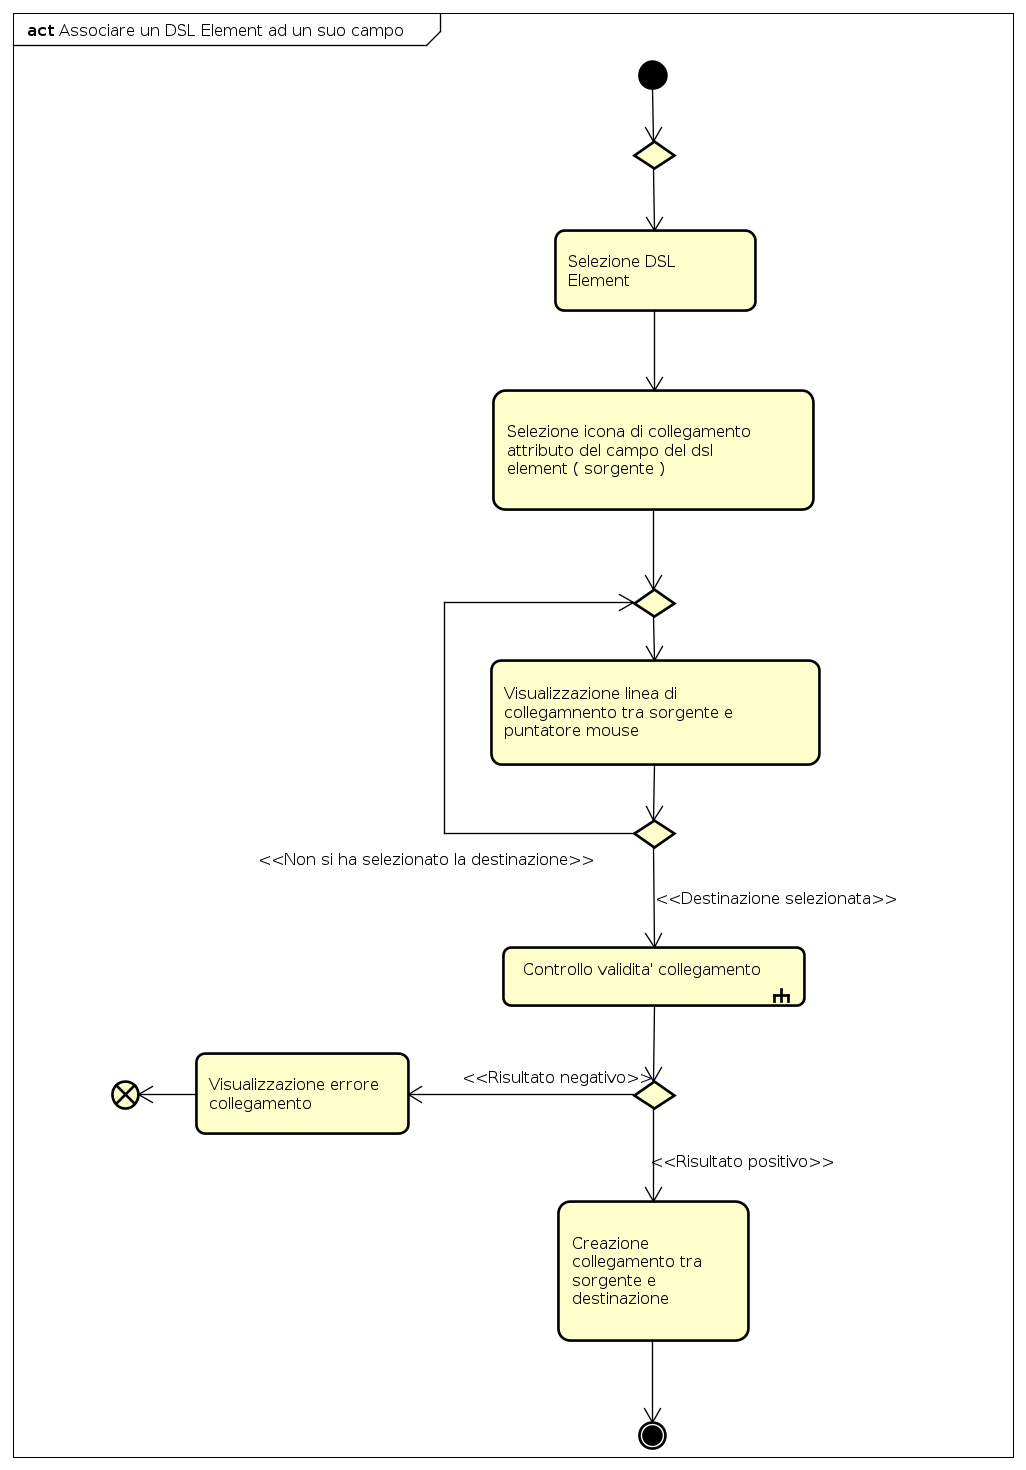
\includegraphics[width=0.8\textwidth]{res/img/associazioneDSLElement.png}
      \caption{Associare un \glossaryItem{DSL} Element ad un campo di un \glossaryItem{DSL} Element}
      \label{fig:diagram_model}
    \end{figure}
    L'utente si trova nella pagina dell'editor e desidera associare ad un attributo di un \glossaryItem{DSL} Element un altro \glossaryItem{DSL} Element. Procede selezionando l'attributo del \glossaryItem{DSL} Element sorgente su cui eseguire l'associazione. Mentre si sposta, visualizza una linea di collegamento tra il puntatore del mouse e la sorgente, che si ferma quando viene scelta una destinazione. Viene effettuato un controllo di validità del collegamento e, in caso di esito positivo il collegamento viene creato, altrimenti l'utente visualizza un messaggio di errore.
    \subsection{Controllo validità collegamento tra due DSL Element}
    \begin{figure}[H]
      \centering
      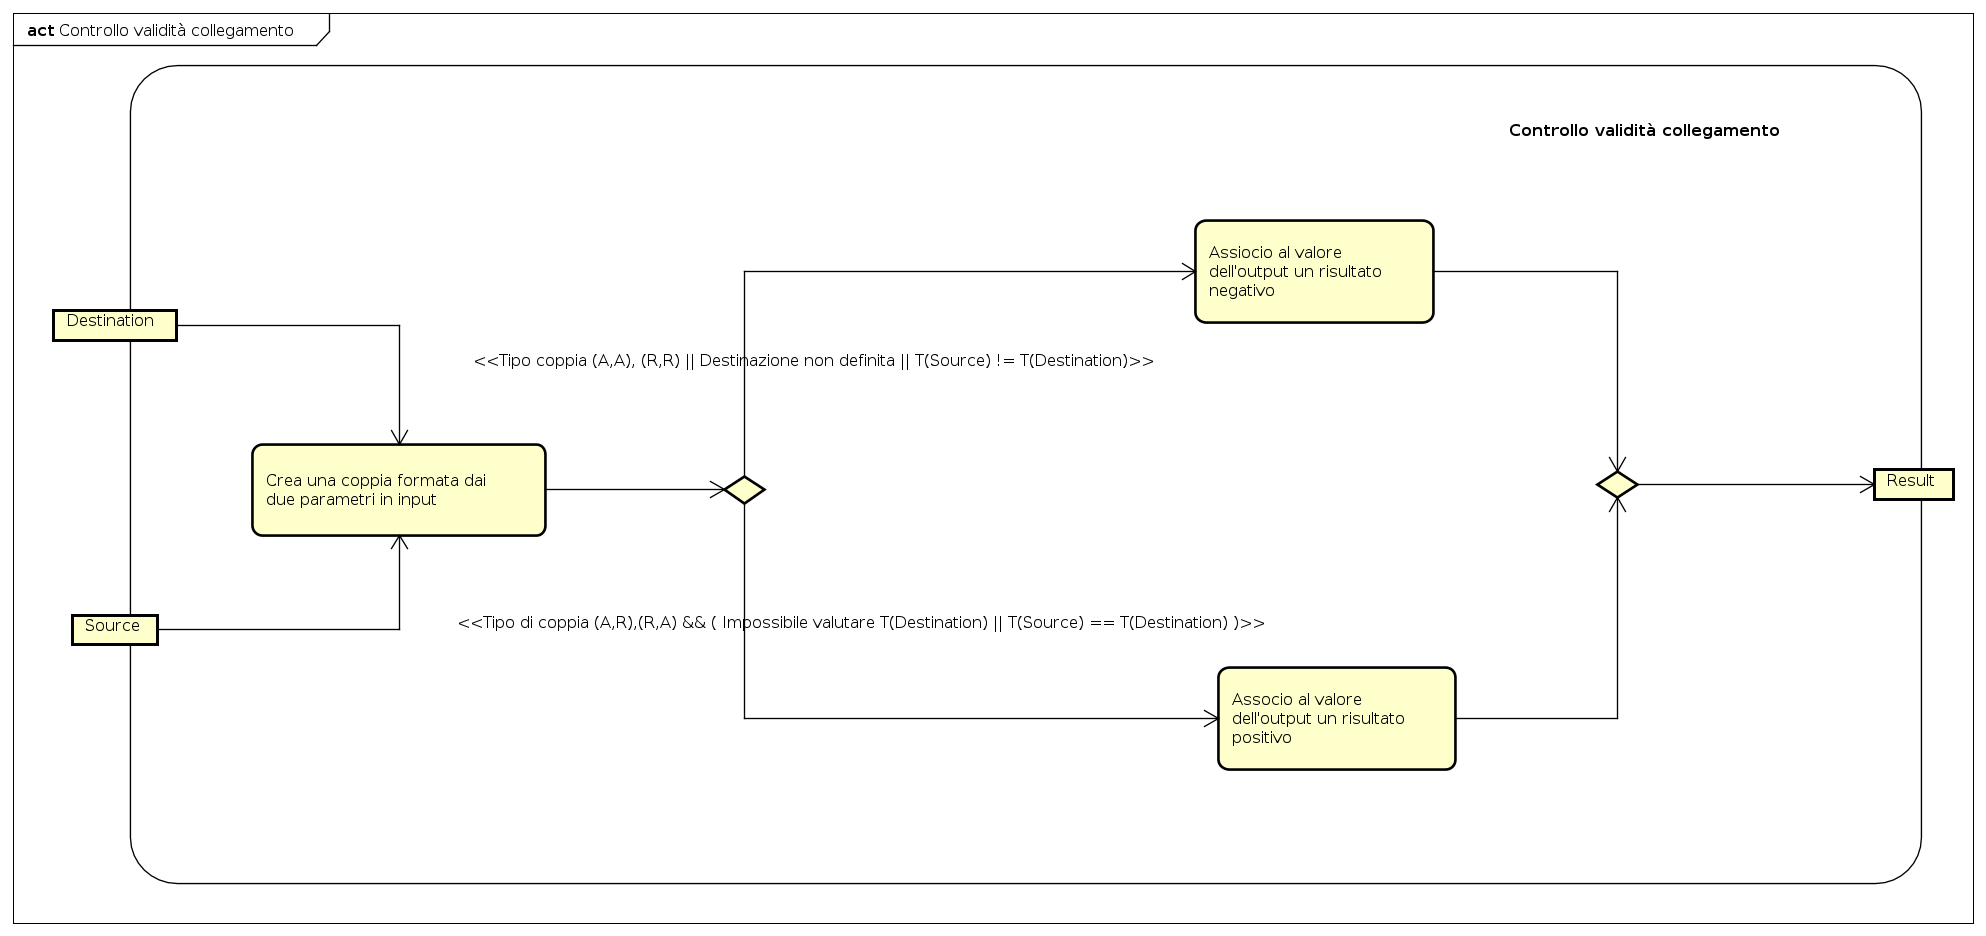
\includegraphics[width=1.1\textwidth]{res/img/controlloCollegamento.png}
      \caption{Controllo validità collegamento tra due \glossaryItem{DSL} Element}
      \label{fig:diagram_model}
    \end{figure}
L'utente si trova nella pagina dell'editor ed ha effettuato un collegamento tra due \glossaryItem{DSL} Element. In questa sotto-attività viene controllata la validità del collegamento, data una coppia (sorgente, destinazione). Questa coppia può essere la combinazione dei tipi \textit{Valore V} o \textit{Riferimento R} (\textit{VV, VR, RV, RR}). Se la coppia è del tipo \textit{VV} o \textit{RR} o l'utente ha cliccato su una sorgente valida ma successivamente in un'area dell'editor non valida, allora il collegamento fallisce. Altrimenti, occorre valutare il tipo della destinazione e della sorgente e confrontarli. Se i tipi sono compatibili (uguali o non confrontabili, ad esempio nel caso del collegamento di un input ad un \glossaryItem{Function Element}), allora il collegamento ha successo, altrimenti no. 
    \subsection{Compilazione campi DSL Element}
    \begin{figure}[H]
      \centering
      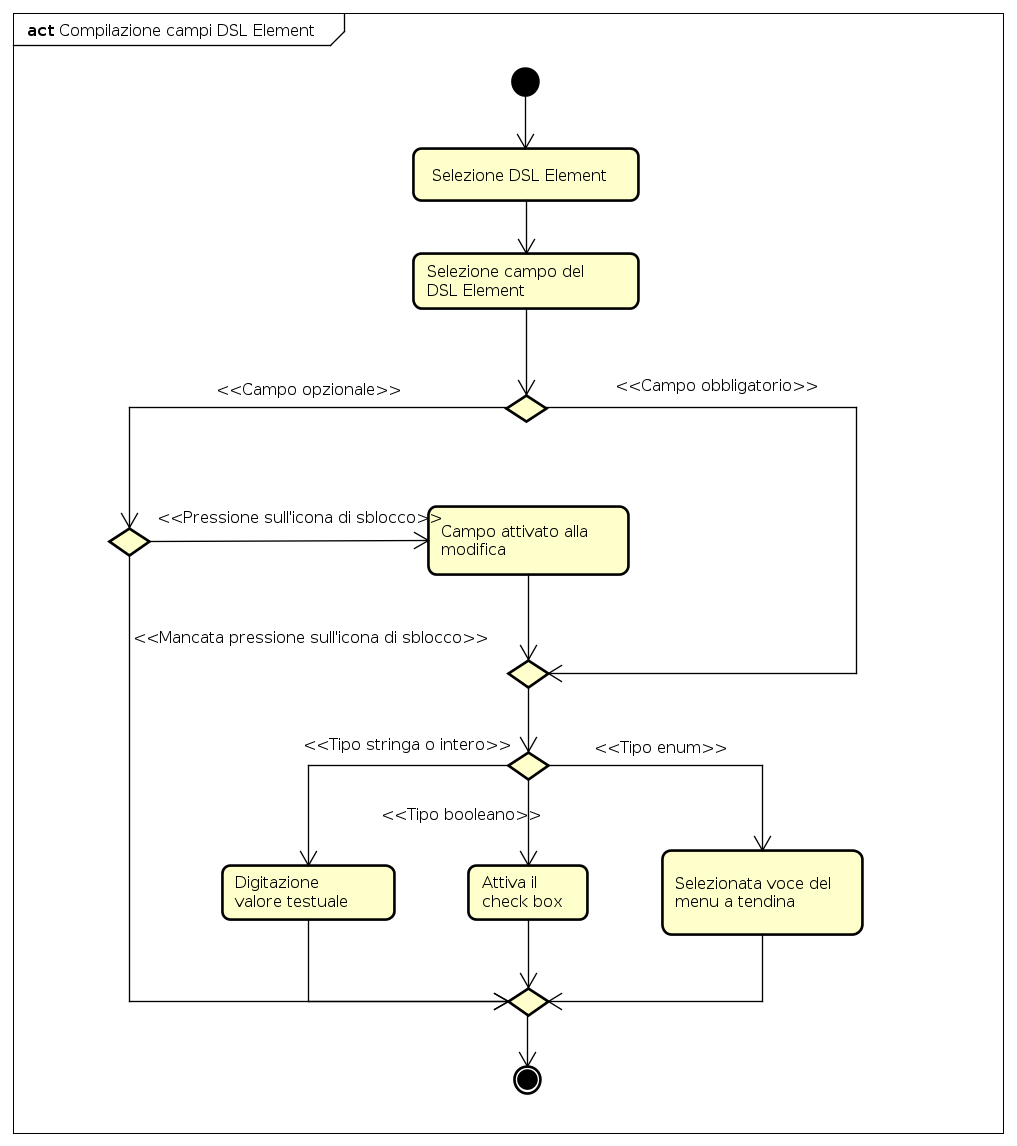
\includegraphics[width=1.1\textwidth]{res/img/compilazioneCampi.png}
      \caption{Compilazione campi \glossaryItem{DSL} Element}
      \label{fig:diagram_model}
    \end{figure}
    L'utente si trova nella pagina dell'editor e desidera impostare un valore per un attributo di un \glossaryItem{DSL} Element. Per farlo seleziona il \glossaryItem{DSL} Element e il campo dell'attributo scelto, se l'attributo è opzionale allora l'utente può ``attivarlo'' facendo pressione sull'icona di sblocco, altrimenti se è obbligatorio procede senza fare nulla. Per impostare un valore, si hanno tre \glossaryItem{casi}: se si tratta di un attributo di tipo stringa o intero, l'utente può digitare il valore testuale desiderato; se si tratta di un tipo booleano, può attivare un check box; infine se si tratta di un tipo enumerazione, può selezionare una voce dal menù a tendina corrispondente al tipo.
    \subsection{Gestione spostamento DSL Element sull'editor}
    \begin{figure}[H]
      \centering
      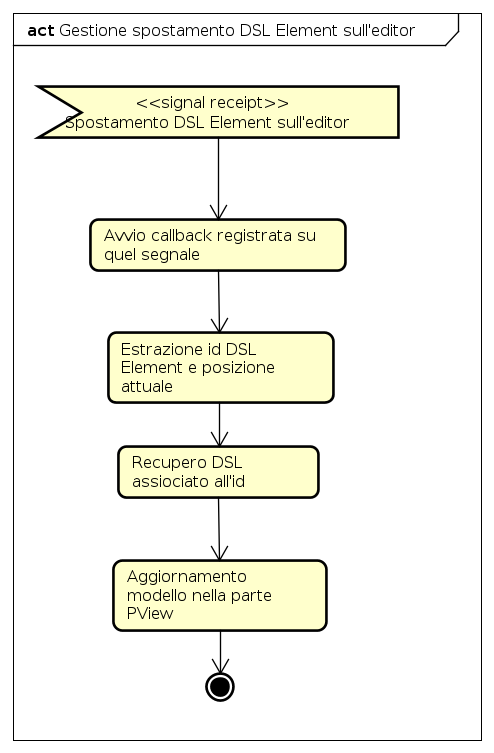
\includegraphics[width=0.5\textwidth]{res/img/spostamentoDSLElement.png}
      \caption{Gestione spostamento \glossaryItem{DSL} Element sull'editor}
      \label{fig:diagram_model}
    \end{figure}
    L'utente si trova nella pagina dell'editor e desidera spostare un \glossaryItem{DSL} Element. Il sistema, avendo a disposizione l'id associato, recupera il \glossaryItem{DSL} Element e mantiene aggiornata la corrispondente \texttt{DSLCreator::PView}.
